\documentclass{article}
\usepackage[top=10mm, bottom=10mm]{geometry}
\usepackage{amsmath}
\usepackage{graphicx}
\usepackage{circuitikz}

\let\vec\mathbf
\newcommand{\myvec}[1]{\ensuremath{\begin{pmatrix}#1\end{pmatrix}}}

\title{Hardware Assignment - Report}
\author{AI24BTECH11031 - Shivram S}
\date{}

\begin{document}
\maketitle

\section{Introduction}

This report details the process of determining the voltage across a 
PT-100 RTD (Resistance Temperature Detector) as a function of temperature.
The least squares method was used to estimate the parameters of the
Callendar-Van Dusen equation.

\section{Collecting Data}

We were provided with the following components
\begin{itemize}
    \item PT-100 Resistance Temperature Detector
    \item Arduino Uno and USB Cable
    \item 10 $\Omega$ resistor
    \item Breadboard
    \item Wires
\end{itemize}

We also made use of the following items from the EE Lab to
control and monitor the temperature
\begin{itemize}
    \item Electric kettle
    \item Digital Thermometer
\end{itemize}

The 10 $\Omega$ resistor and the PT-100 were connected in series
between the 5V output pin and the ground pin of the Arduino to create
a voltage divider. The other pin of the PT-100 is connected to the
A0 pin of the Arduino to measure the voltage across the PT-100.

\begin{figure}[h!]
    \centering
    \begin{circuitikz} \draw
        (0,0) to[battery1, l=$5\ V$, invert] (0,2)
        to[R, l^=$10\ \Omega$] (3,2) to[short, -o] (5,2) node[right] {A0 (Arduino)};
        \draw (3,2) to[R, l^=$P\ \Omega$ (PT-100)] (3,0)
        -- (0,0);
        \draw (3,0) to[short, -o] (5,0) node[right] {GND (Arduino)};
    \end{circuitikz}
\end{figure}

The PT-100 was immersed in an electric kettle filled with water, and a digital
thermometer was used to measure the temperature. The C++ code used to drive the
Arduino can be found in the appendix.

The kettle was turned on for some time, and then turned off. Once the reading of
the digital thermometer becaome stable, a reading was taken, and the Temperature
was increased again. A total of 32 readings were taken over a range of temperatures
from 27.3 $^\circ$C to 95 $^\circ$C.

\begin{figure}[h!]
\centering
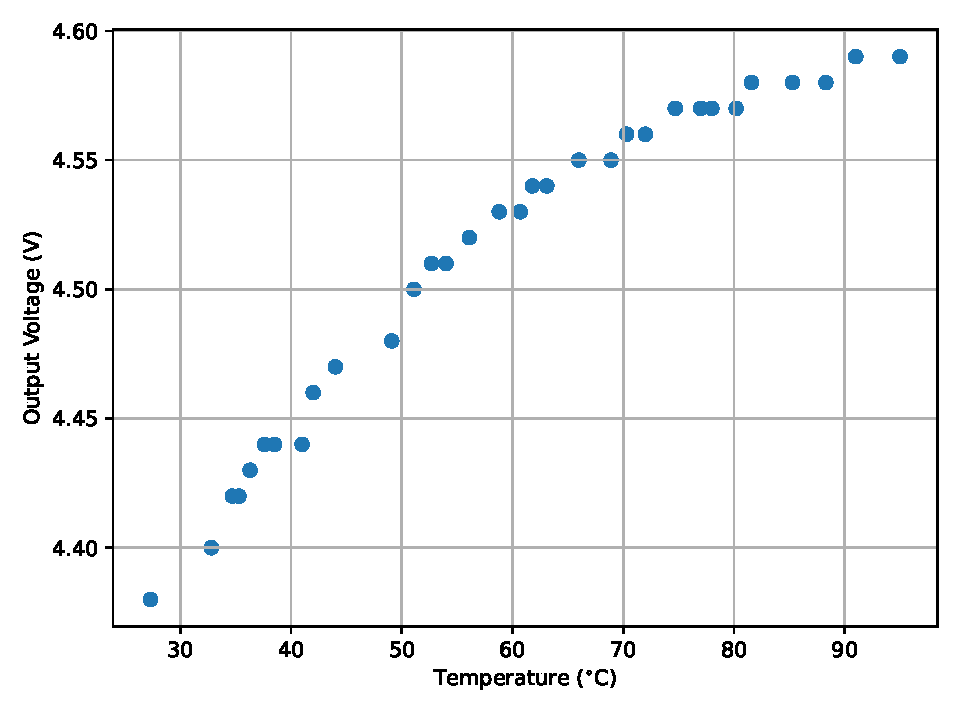
\includegraphics[width=0.75\linewidth]{figs/data}
\end{figure}

7 points were randomly chosen from the data set to form the
validation set. The remaining 25 points were put in the
testing set.

\section{Model}

We use the Callendar-Van Dusen equation to model the voltage across the PT-100
as a quadratic function fo temperature.

\begin{align*}
    V(T) &= V(0)(1 + AT + BT^2) \\
    c &= \vec{n}^\top \vec{x} \\
\end{align*}

where

\begin{align*}    
    c &= V(T), \vec{n} = V(0)\myvec{1 \\ A \\ B}, \vec{x} = \myvec{1 \\ T \\ T^2}
\end{align*}

We can write the equation in matrix form as

\begin{align*}
    \vec{X}^\top \vec{n} = \vec{C}
\end{align*}

where

\begin{align*}
    \vec{X} = \myvec{1 & 1 & \dots & 1 \\ T_1 & T_2 & \dots & T_n \\ T_1^2 & T_2^2 & \dots & T_n^2},
    \vec{C} = \myvec{V(T_1) \\ V(T_2) \\ \vdots \\ V(T_n)}
\end{align*}

In the least squares method, we try to minimize the squared loss function
\begin{align*}
 L(\vec{n}) = \Vert \vec{X}^\top\vec{n} - \vec{y} \Vert^2
\end{align*}

where $\vec{y}$ is the vector of voltage readings. This can be done by finding 
the point at which the gradient of the loss function is zero.

\begin{align*}
    \frac{dL(\vec{n})}{d\vec{n}} = \vec{0}
\end{align*}

The solution which minimizes the loss function is given by

\begin{align*}
    \vec{n} = \left( \vec{X}^\top \vec{X} \right) \vec{X}^\top \vec{y}
\end{align*}

The solution may also be calculated using singular value decomposition.
This method reduces rounding errors caused by smaller numbers, and also
handles under-determined systems better.

In singular value decomposition, we write $\vec{X}$ in terms of three matrices - 
two orthogonal matrices $\vec{U}$ and $\vec{V}$, and a diagonal matrix $\vec{\Sigma}$.

\begin{align*}
    \vec{X} = \vec{U}\vec{\Sigma}\vec{V}^\top
\end{align*}

We can then write $\vec{n}$ as 

\begin{align*}
    \vec{n} = \vec{V}\vec{\Sigma}^\dagger \vec{U}^\top \vec{y}
\end{align*}

The Python program in the appendix computes the value of $\vec{n}$ using
the least squares method and also plots the voltage as a function of temperature.

\begin{align*}
    \vec{n} = \myvec{4.1600\\ 9.132 \times 10^{-3} \\ -4.9232 \times 10^{-5}}
\end{align*}

The approximate model is given by 

\begin{align*}
    V(T) = 4.1600 + (9.132 \times 10^{-3})T + (-4.9232) \times 10^{-5})T^2
\end{align*}

\begin{figure}[h!]
\centering
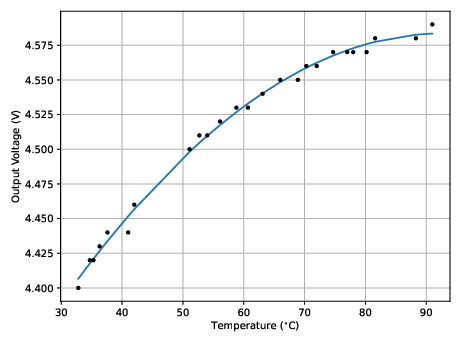
\includegraphics[width=0.75\linewidth]{figs/train}
\end{figure}

The model can be validated by using the validation data set.

\begin{figure}[h!]
\centering
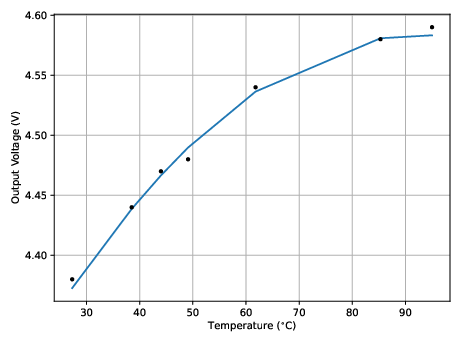
\includegraphics[width=0.75\linewidth]{figs/valid}
\end{figure}


\end{document}